\documentclass[]{article}
\usepackage{lmodern}
\usepackage{amssymb,amsmath}
\usepackage{ifxetex,ifluatex}
\usepackage{fixltx2e} % provides \textsubscript
\ifnum 0\ifxetex 1\fi\ifluatex 1\fi=0 % if pdftex
  \usepackage[T1]{fontenc}
  \usepackage[utf8]{inputenc}
\else % if luatex or xelatex
  \ifxetex
    \usepackage{mathspec}
  \else
    \usepackage{fontspec}
  \fi
  \defaultfontfeatures{Ligatures=TeX,Scale=MatchLowercase}
\fi
% use upquote if available, for straight quotes in verbatim environments
\IfFileExists{upquote.sty}{\usepackage{upquote}}{}
% use microtype if available
\IfFileExists{microtype.sty}{%
\usepackage[]{microtype}
\UseMicrotypeSet[protrusion]{basicmath} % disable protrusion for tt fonts
}{}
\PassOptionsToPackage{hyphens}{url} % url is loaded by hyperref
\usepackage[unicode=true]{hyperref}
\hypersetup{
            pdfborder={0 0 0},
            breaklinks=true}
\urlstyle{same}  % don't use monospace font for urls
\usepackage[margin=1in]{geometry}
\usepackage{graphicx,grffile}
\makeatletter
\def\maxwidth{\ifdim\Gin@nat@width>\linewidth\linewidth\else\Gin@nat@width\fi}
\def\maxheight{\ifdim\Gin@nat@height>\textheight\textheight\else\Gin@nat@height\fi}
\makeatother
% Scale images if necessary, so that they will not overflow the page
% margins by default, and it is still possible to overwrite the defaults
% using explicit options in \includegraphics[width, height, ...]{}
\setkeys{Gin}{width=\maxwidth,height=\maxheight,keepaspectratio}
\IfFileExists{parskip.sty}{%
\usepackage{parskip}
}{% else
\setlength{\parindent}{0pt}
\setlength{\parskip}{6pt plus 2pt minus 1pt}
}
\setlength{\emergencystretch}{3em}  % prevent overfull lines
\providecommand{\tightlist}{%
  \setlength{\itemsep}{0pt}\setlength{\parskip}{0pt}}
\setcounter{secnumdepth}{0}
% Redefines (sub)paragraphs to behave more like sections
\ifx\paragraph\undefined\else
\let\oldparagraph\paragraph
\renewcommand{\paragraph}[1]{\oldparagraph{#1}\mbox{}}
\fi
\ifx\subparagraph\undefined\else
\let\oldsubparagraph\subparagraph
\renewcommand{\subparagraph}[1]{\oldsubparagraph{#1}\mbox{}}
\fi

% set default figure placement to htbp
\makeatletter
\def\fps@figure{htbp}
\makeatother

\usepackage{float}
\usepackage{titling}
\usepackage{caption} 
\usepackage{amsmath}
\usepackage{booktabs}
\captionsetup[table]{skip=8pt}
\usepackage{abstract}
  \renewcommand{\abstractnamefont}{\normalfont\large\bfseries}
\usepackage{booktabs}
\usepackage{longtable}
\usepackage{array}
\usepackage{multirow}
\usepackage{wrapfig}
\usepackage{float}
\usepackage{colortbl}
\usepackage{pdflscape}
\usepackage{tabu}
\usepackage{threeparttable}
\usepackage{threeparttablex}
\usepackage[normalem]{ulem}
\usepackage{makecell}
\usepackage{xcolor}

\author{}
\date{\vspace{-2.5em}}

\begin{document}

\begin{flushleft}
\LARGE{\textbf{Country Level Indicators of Suicide Risk:\\ Data Analysis \& Decision Support for Policy Makers}}\\
\vspace*{3\baselineskip}
\Large{Project Report: Georgia Tech ISyE 6414 - Dr. Yajun Mei}\\
\vspace*{3\baselineskip}
\large{\textbf{Team Members}}\\
Samuel Garcia - samgarciajr@gatech.edu (611)\\
Michael Szostak - mszostak3@gatech.edu (302)\\ 
Osman Ghandour - oghandour3@gatech.edu (885) \\ 
Peter Williams - pwilliams60@gatech.edu (374)\\
\vspace*{2\baselineskip}
\large{\textbf{Report Date}}\\
April 21, 2020
\newpage
\end{flushleft}

{
\setcounter{tocdepth}{3}
\tableofcontents
}
\newpage

\begin{abstract}
\bigskip

Suicide is a complex worldwide problem that has many causes. This report aims to highlight trends related to country-level measures of suicide globally. The researchers utilize open source data from the World Health Organization and other non-governmental bodies to develop an inferential statistical model. The model considers country level data related to the wealth, culture, and specific efforts to improve mental health. The model is developed through the implementation of a couple of key algorithms and variable transformations.

Based on our analysis we recommend countries to consider establishing an authoritative agency that can manage the investigation, formulation, and implementation of a national suicide prevention strategy. Additionally, policy makers should consider implementing measures designed to mitigate the harmful use of alcohol. We also recommend investment in research to better understand potential relationships between income instability, income protection and suicide at the individual level. 

An overview of potential limitations of our research in context of the scope of the data we collected, and the methodologies we employed is provided. This overview is meant inform interpretation of key variables of interest in our model, as well as providing commentary on the limitations of using aggregate data to make inferences at local or regional levels.  
   
\end{abstract}

\section{Research Motivation}\label{research-motivation}

Suicide is a complex societal problem with multiple social,
psychological, biological, and cultural factors. It is one of the top 20
leading causes of death in the world for all ages {[}4{]}. An estimated
one million people die annually from suicide, i.e., a global mortality
rate of \(16\) per \(100,000\), or one death every \(40\) seconds
{[}4{]}. Due to the interactions of so many factors, suicide has no
singular cause.\\
Though it might seem intuitive to categorize suicidal ideation,
attempted suicide, and completed suicide as strictly a psychiatric or
medical issue or a mental illness, not all who commit suicide are
mentally ill. Mental illness is often not clearly distinguishable from
normal distress {[}5{]}. Stressful experiences, such as exposure to
trauma, the death of a loved one, a job loss, a change in physical
health or relationships and individual characteristics and behaviors are
also associated with suicide {[}6{]}.

\subsection{Global Trends in Suicide
Epidemiology}\label{global-trends-in-suicide-epidemiology}

Suicide is the 15th leading cause of death worldwide, with over 75\% of
suicides occurring in low-income and middle-income countries {[}19{]}.
Poverty, particularly in the form of worse economic status, diminished
wealth, and unemployment is associated with suicide {[}19{]}. Poverty
may be defined in terms of deprivation across the multiple dimensions of
life, such as education, health, or housing {[}20{]}. Both chronic
poverty and acute economic events, such as crop failure, constitute
possible risk factors for suicidal ideations and behaviors {[}19{]}.

Poverty, unemployment, illiteracy, lack of civic facilities, poor access
to health facilities, the absence of health insurance or of welfare are
factors that adversely impact upon the overall mental health status of
the population {[}21{]}. In developing countries, the interval between
onset of suicidal ideation and the act of suicide is frequently
overlooked---partly because of ignorance but also because families and
subjects do not know where to seek help. Even when they do realize
something is wrong, they lack resources to seek help. {[}21{]}

To underscore the complex nature of the suicide problem, and to show how
causes of suicide can vary between countries, we contrast the situations
in Zimbabwe and Russia. Zimbabwe has suffered endemic poverty,
hyperinflation, and high unemployment for years. On the other hand,
Russia's levels of alcohol consumption are among the highest in the
world. Though their underlying conditions appear to be markedly
different, both nations suffer from high rates of suicide.

\subsubsection{Case Study: Economics -
Zimbabwe}\label{case-study-economics---zimbabwe}

Endemic poverty, hyperinflation, and an unemployment rate of over 90\%
{[}7{]} are among the economic and social problems plaguing Zimbabwe,
where political crisis coupled with failed economic policy have led to
its decline. Zimbabwe's economic woes are often attributed to the
policies of former dictator Robert Mugabe. Post Mugabe, Zimbabwe
continues to deal with debt issues, difficulty attracting foreign
investment, and currency instability.

The WHO estimates that 19 persons per 100k take their own life
deliberately in Zimbabwe per annum (2019). Of the 166 countries in our
study, Zimbabwe ranks 13th in the world for suicides per capita.

\emph{Figure 1: Suicide Rate in Africa (annual persons per 100k
population)}

\begin{center}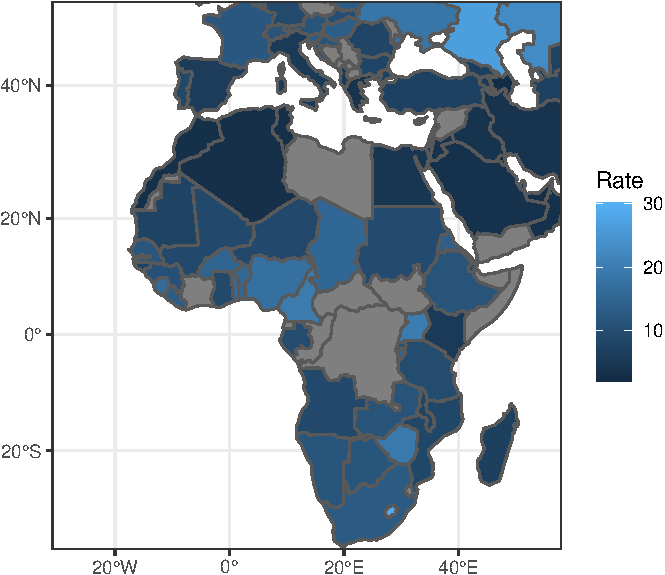
\includegraphics{Project_Report_files/figure-latex/africa_map_plot-1} \end{center}

\emph{Sourced from the World Health Organization report: ``Suicide: Key
Facts, 2019'' and the WorldBank Economic Profile of the Country of
Zimbabwe}

\subsubsection{Case Study: Alcohol Abuse -
Russia}\label{case-study-alcohol-abuse---russia}

In general, there is no single factor responsible for the suicide rate.
Globally however, harmful use of alcohol is among the major risk factors
for suicide.

A study published in The Lancet found that global alcohol consumption
saw an increase of about 70\% from 1990 to 2017, going from about 21
billion liters of pure alcohol to 35.7 billion liters of pure alcohol
{[}22{]}. Countries that have higher rates of alcohol use generally also
have higher rates of suicide. Current evidence indicates an association
between alcohol dependence and impulsive suicide attempts {[}4{]}.

Alcohol use disorder (AUD), defined in the WHO's International
Classification of Diseases, is a chronic disease characterized by
compulsive alcohol consumption, loss of control over of alcohol intake,
and negative emotional state when not consuming alcohol. Alcohol
intoxication can increase dysphoria, cognitive dysfunction, impulsivity
and suicidal ideation. People have approximately seven times increased
risk for a suicide attempt soon after drinking alcohol, and this risk
further increases to 37 times after heavy use of alcohol {[}12{]}. Risk
of suicidal ideation, suicidal attempts and completed suicide are each
increased by 2--3 times among those with Alcohol Use Disorders (AUD) in
comparison with the general population {[}12{]}.

In Russia, the prevalence of AUD is about 4.7\%, meaning that almost
1-in-20 suffer from alcohol dependence {[}8{]}. Alcoholism has been a
problem because drinking is not only pervasive, but also a socially
acceptable behavior in Russian society. The WHO estimates that 27
persons per 100k take their own life deliberately in Russia per annum
(2019). Of the 166 countries in our study, Russia ranks 3rd in the world
for suicides per capita.

\emph{Figure 2: Suicide Rate in Russia (annual persons per 100k
population)}

\begin{center}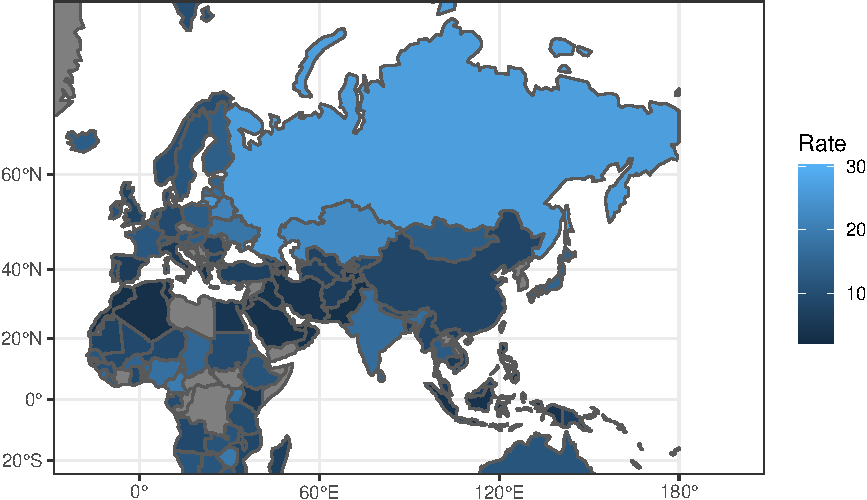
\includegraphics{Project_Report_files/figure-latex/russia_map_plot-1} \end{center}

\emph{Sourced from the World Health Organization report: Suicide: Key
Facts, 2019}

\section{Variables \& Data Sources}\label{variables-data-sources}

Due to the sheer number of potential factors associated with suicide and
the complex nature of the relationships between them, we wanted to
identify those that were best associated with suicide rates at the
country level. We chose to limit our study to a small set of factors
that could be controlled for and acted upon via policy interventions.
The domains from which we drew the factors, had to be broad enough to
reasonably represent as many of the potential causes or mitigators of
suicide as possible.

Among the domains in consideration were lifestyle, medical/mental
health, economic, and suicide-focused policy. The core dataset we plan
to rely on comes directly from the World Health Organization {[}3{]}
(\emph{WHO}). The key measure of interest for our study is the
age-standardized suicide rate by country, which is defined as a weighted
average of the age-specific mortality rates per 100,000 persons, where
the weights are the proportions of persons in the corresponding age
groups of the WHO standard population, see the Appendix section for
details on how this is estimated. Estimates of age-standardized suicide
rates were taken in the year with the most recent available data for
each country from the \emph{WHO}.

In addition to the core suicide rate statistics provided above, we
append country-level data from ancillary data sources. Health
Expenditure and GDP per capita were chosen to reflect the resources that
a country has its disposal to reduce the suicide rate. Liters of Alcohol
per capita was chosen to account for an aspect of culture (alcohol
consumption) that the media often links to mental health outcomes. The
prevalence of a suicide prevention strategy, the number of
psychiatrists, and the number of mental hospitals were chosen to reflect
how a country has deployed its resources to improve mental health
outcomes. The female/male labor participation ratio was included to
control for this aspect of a country's culture. The data for these
variables along with the suicide rate variable was available for 166
countries.

Below is the full set of considered independent variables with
corresponding source:

\begin{itemize}
  \item Current Health Expenditure as a percentage of GDP: *World Health Organization*  
  \item Labor force participation rate, female to male ratio: *United Nations Development Programme*
  \item GDP per capita, adjusted by Purchasing Power Parity: *World Bank*
  \item Liters of Alcohol consumption per capita: *World Bank*
  \item Presence of a Suicide Prevention Strategy: *World Health Organization*
  \item Psychiatrists in mental health, per 100,000 population: *World Health Organization*
  \item Mental hospitals, per 100,000 population: *World Health Organization*
\end{itemize}

Note that more detailed descriptions of the data and the source links
can be found in the \emph{Appendix}.

\section{Modeling \& Assumptions}\label{modeling-assumptions}

We developed a multiple linear regression model to infer properties
about how a handful of socioeconomic and cultural indicators impact
suicide rates. An important distinction is that the model is intended to
be used for inferential, rather than predictive purposes. Our objective
is to discover relationships between variables to inform relevant public
policy and future research in the area.

The first step in developing the model was to transform the outcome
variable. This transformation (Box-Cox) was used to make the outcome
variable `more normal', and it helped to characterize relationships
between variables in our data. The next step was to remove outliers. We
used regression diagnostics and visual data exploration to identify
unusual data points. Brief qualitative research was then conducted on
the country represented by each point to confirm whether or not the
point should be removed. After the removal of the outlier points, we
utilized a stepwise algorithm to identify which variables should be
included in our model. This `automatic' procedure yielded the set of
variables that we would analyze more closely.

The following variables were selected and included in our model: labor
force participation rate (female-male ratio), GDP per capita (PPP),
liters of alcohol consumption per capita, and the prevalence of a
national suicide prevention strategy. The algorithm excluded the
following variables from the model: current health expenditure as a
percentage of GDP, the number of psychiatrists working in the mental
health sector (per 100k pop.), and the number of mental hospitals (per
100k pop.).

The final step in the development of our model was to implement an
iterative algorithm that adjusted the weights for each of our data
points (Iteratively Reweighted Least Squares). This allowed us to
further limit the influence of outliers on our data.

In the development of our model, we relied on a few assumptions about
the quality of our data. The first is regarding GDP per capita, which is
assumed to be an appropriate indicator to reflect the wealth of a
country. The second relates to the prevalence of a national suicide
prevention strategy. It is assumed that the presence of such a strategy
is indicative that the country has taken the time to develop a
comprehensive and data driven approach to suicide, based on solid
evidence. We also assume that the liters of alcohol consumed per capita
reflects the tendency for individuals in the given country to consume
excessive amounts of alcohol.

To develop models utilized in this report we relied on the based
functionality provided in the \emph{R} language. Further details can be
found in the appendix.

\section{Quantifying Impact of Measures on
Suicide}\label{quantifying-impact-of-measures-on-suicide}

Our model allows the data analyst to describe the relationships between
country-level indicators and measures and suicide rates globally. Armed
with a descriptive model of suicide rates, decision-makers can quantify
the relationships between these measures to support insight for their
health related planning activities. However, data-driven insights
derived from this model and the data sources highlighted in this report
should be considered in context of specific country-level impacts not
considered in this report. As policy makers infer correlations of
country-level measures and indicators with suicide rates there is a need
to continue to engage subject-matter-experts in the field to draw on
their knowledge and experience. Our intention is to provide some initial
context and decision support for policy makers managing health related
planning globally and at the country level, but the limitations of our
research and methodology highlight the ongoing need for data-driven
insights to be utilized in context of other research available, as well
as the domain knowledge of practitioners, health professionals,
scientists, and policy makers among others.

To highlight the need for a holistic approach to gathering data-driven
insights, and incorporating domain knowledge of subject matter experts,
we describe a basic framework for potentially incorporating insights
from our model into a policy decision-making process:

\begin{table}[H]
\centering 
\caption{Framework: Identifying, Describing and Monitoring Country Level Indicators to Support Decision-Making}
\
\begin{tabular}{p{7cm}p{9cm}}  
\hline  
   Area of Focus  & Decision Support  \\   
\hline 
 Identifying \& Quantifying Measures and Indicators of Country Level Suicide Rates &  Using a model to describe the relationships between country-level indicators and suicide rates to help policy makers identify what variables are important and putting context around how to monitor them \\   
 \hline 
Incorporating Domain Knowledge and Expertise of Subject Matter Experts & Allows policy makers to correlate indicators with country-level suicide related outcomes in context of qualitative insights from experts in the field \\   
\hline 
Insight Gathering, Analysis and Support Policy Maker Decisions & Integrating data and insights and providing inital context to help policy makers to frame longer term health planning activities and policies \\
\hline 
\end{tabular} 
\end{table}

In context of providing exemplary decision-support for health related
planning activities we discuss some interesting relationships we
identified between country-level suicide rates and the descriptor
variables we selected in the following sections.

\subsection{Quantifying Impact: Income, GDP per
person}\label{quantifying-impact-income-gdp-per-person}

A key insight that surfaced during the modeling process was the presence
of a significant relationship between a measure of income (here defined
as the country-level GDP per person) and country level suicide rates.
Countries with lower per person income, tend to have higher incidence of
suicide. To explore this relationship further, we look at the impact of
income, or per-person GDP, on a country's suicide rate controlling for
the other key factors in our model including alcohol consumption, the
female-male labor participation rate, and the presence of a
country-level suicide prevention strategy.

When controlling for these variables, we found that an approximate 10\%
increase in income (or GDP per-person) corresponded to a 2\% decrease in
suicide rate at the country level for the typical country. The following
plot highlights the sensitivity of income to suicide rates based on
results from our model:

\emph{Figure 3: Expected Country-Level Suicide Rate vs.~Income (GDP
per-person)}

\begin{center}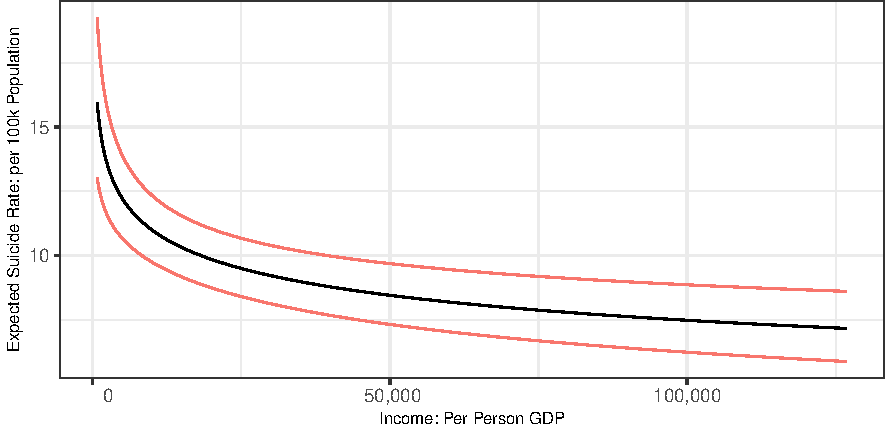
\includegraphics{Project_Report_files/figure-latex/agdp_plot-1} \end{center}

\emph{Note: Expected rate with 95\% confidence intervals for the typical
country (i.e.~holding other variables in model identified fixed at the
`sample mean').}

\subsection{Quantifying Impact: Alcohol
Consumption}\label{quantifying-impact-alcohol-consumption}

A key insight that surfaced during the modeling process was the presence
of a significant relationship between a measure of alcohol abuse, liters
of consumption per year, and suicide country level suicide rates. As
might be expected, countries with higher levels of alcohol consumption
income in our data, tended to have higher incidence of suicide when
controlling for other variables in our model. Based on our estimates, an
approximate 4\% increase in alcohol consumption corresponded to an
expected 2\% increase in suicide rate for countries where adults, on
average, consume more than 4 liters of alcohol per year.

Another thing to note from our data analysis, is that alcohol
consumption was the most impactful and significant indicator of
country-level suicide rate in our model. The illustrate the estimated
impact, the following plot highlights the sensitivity of alcohol
consumption to suicide rates based on results from our model:

\emph{Figure 4: Expected Country-Level Suicide Rate vs.~Liters of
Alcohol Consumer Per Year (pp)}

\begin{center}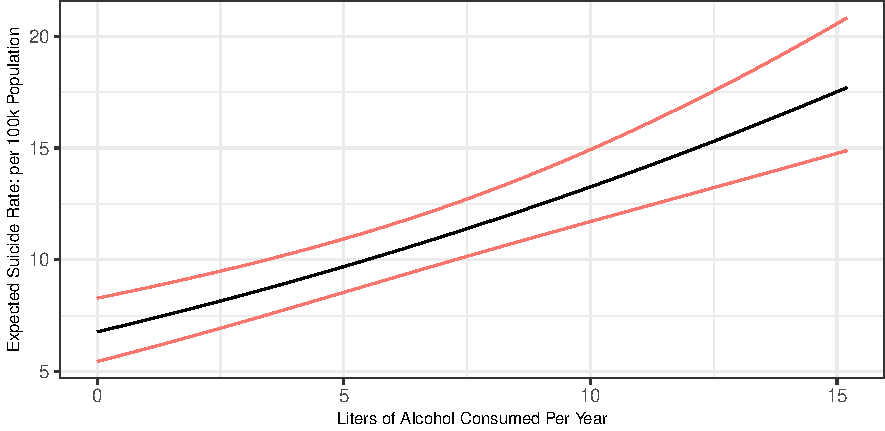
\includegraphics{Project_Report_files/figure-latex/a_alc_plot-1} \end{center}

\emph{Note: Expected rate with 95\% confidence intervals for the typical
country (i.e.~holding other variables in model identified fixed at the
`sample mean').}

This sensitivity analysis highlights the strong relationship between
these variables, which isn't an entirely novel relationship we
discovered. Our brief case study of suicide in Russia was meant to
provide some discussion of the real impact alcohol consumption.

\subsubsection{Quantifying Impact: The Presence of A National Suicide
Strategy}\label{quantifying-impact-the-presence-of-a-national-suicide-strategy}

A key variable we wanted to control for in our model was an indicator of
a country having a national suicide prevention strategy in place. Based
on data criteria from the \emph{WHO}, we measured the impact of having a
stand-alone national suicide prevention strategy. According to the
\emph{WHO} the categorical criterion for the presence of a national
suicide strategy was that, in order to be considered, as country's
planplan have been stand-alone, and not be integrated into another plan.

As we looked at the data, we found that the presence of a suicide
prevention strategy was more likely to be associated with countries
struggling with suicide prevention overall. Some of these countries
included Guyana, Lithuania, Suriname, Belarus and South Korea.

Based on our estimates from our model, countries that have implemented a
suicide prevention strategy have a 26\% higher incidence of suicide
nationally as shown below:

\emph{Figure 5: Expected Country-Level Suicide Rate vs.~The Presence of
A National Suicide Strategy}

\begin{center}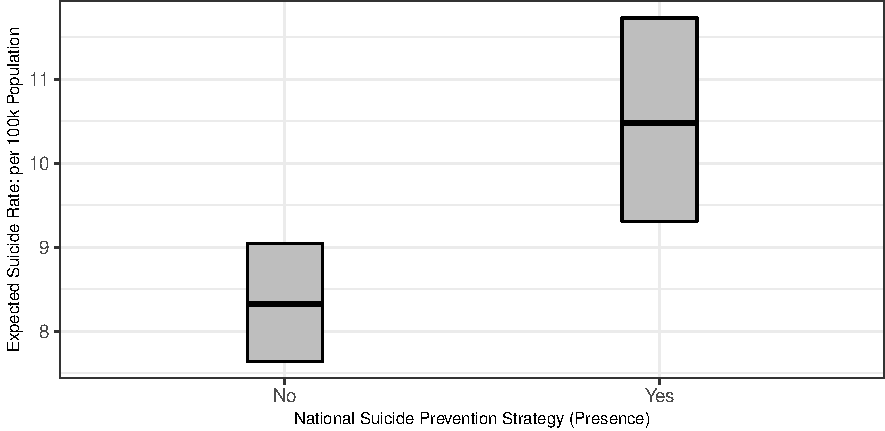
\includegraphics{Project_Report_files/figure-latex/sstrat_plot-1} \end{center}

\emph{Note: Expected rate with 95\% confidence intervals for the typical
country (i.e.~holding other variables in model identified fixed at the
`sample mean').}

While it may seem unintuitive that countries with with a suicide
prevention strategy have higher rates, it should not be inferred or
interpreted from our model that having a national suicide prevention
strategy leads to incidence of suicide rates overall. It may be
understood that the institution of this strategy may be a `reactive'
decision, that is, the presence of a strategy has been instituted as a
result of high incidence. As a result, we wanted to ensure we were
incorporating this variable in our model as both a control for
estimating other effect, and for providing context for countries with
high rates of suicide otherwise.

\section{Recommendations and Decision
Support}\label{recommendations-and-decision-support}

For the selected inputs chosen in the model, there are corresponding
recommendations for each input. The following sections go over
recommendations for each model input:

\subsection{Suicide Prevention
Strategy}\label{suicide-prevention-strategy}

National Suicide prevention strategies have been implemented in many
countries to combat suicide. Many have found their own way of handling
the problem, but there was not widespread acceptance and organizational
response to the problem until recently. In 1993 The United Nations
created a task force which teamed up with the WHO to put together a
study on the causes, preventative, and rehabilitative measures of
suicide, and which culminated with the release of a report in 1996
called ``Prevention of suicide: guidelines for the formulation and
implementation of national strategies'' {[}24{]}. Before this, Finland
was the only nation which had a national program for suicide prevention.

These guidelines were followed to varying degrees by different countries
or local municipalities. The 1996 study was followed up with another
study in 2018 {[}10{]} which contained updated recommendations and
findings since 1996. For instance, the intersection of biological,
psychological, social, environmental, and cultural factors which
influence suicide, as well as successfully implemented policies from
which countries which had a national suicide prevention program
implemented. The 2018 study contained a list of all countries with ``a
stand-alone national suicide prevention strategy (NSPSs) adopted by the
government'' {[}10{]}. For our research, the indicator variable was
sourced from this list.

We found that countries that have put a national suicide prevention
strategy in place, tend to have higher incidence of suicide rates
overall, this may be reactionary in nature. If a country has high
suicide rates then more attention is paid to the issue and programs are
put in place to combat it. Since most National suicide programs have
only been emplaced in the last two decades, this may explain the
counterintuitive trend observed. However, it is still advised to have a
national strategy to address suicide.

Government policy to combat suicide allows for the ``development and
strengthening surveillance (of at-risk groups), and to provide and
disseminate information'' {[}10{]} on at-risk individuals to inform
action. An implementation of a NSPS in Scotland called ``Choose Live''
decreased suicide rates by 20\% over 10 years. This sort of improvement
in suicide rates after implementing is implied in the 2018 report and
lends to the recommendation that national strategies should be
implemented.

Developing countries are recommended to take advantage of online
resources for policy planners like MiNDbank a website created by the WHO
with recommendations on mental health issues {[}9{]}. Countries still
should consider establishing an authoritative agency, tasked with the
continued investigating, formulating, and implementing of a National
Suicide Prevention Strategy. It should follow actions like those below
from countries with success in reducing suicide {[}25{]}:

\begin{itemize}
  \item Reduce access to means and methods of suicide 
  \item View suicide as a psychological mistake
  \item Improve medical, psychological, and psychosocial initiatives
  \item Distribute knowledge about evidence-based methods for reducing suicide
  \item Raise skill levels among staff and other key individuals in the care services
  \item Perform “root cause” or event analyses after suicide
  \item Support voluntary organizations 
  \item Promote public awareness campaigns highlighting the prevalence of suicide
\end{itemize}

National strategies should not replace existing frameworks already in
place in local government either. By changing public perceptions,
reducing the stigmas associated with seeking help, and coming up with
national strategies to combat suicide, the rate of suicide can be
reduced.

\subsection{Alcohol Intake}\label{alcohol-intake}

Suicide is a complex societal problem with no singular cause. However,
harmful use of alcohol is among the major risk factors for suicide.
Policy makers should consider implementing measures designed to mitigate
the harmful use of alcohol as a means of reducing the rate of suicide.
According to the WHO, among the policy interventions that have proven
effective at reducing the harmful use of alcohol are varied. One is to
increase the price of alcohol via taxation, which is implemented
successfully in states such as Utah. Another is to enact and enforce
restrictions on alcohol advertising (across multiple types of media),
out of sight out of mind. And finally, enact and enforce restrictions on
the physical availability of retailed alcohol (via reduced hours of
sale), for example many ``dry states'' do not serve alcohol on Sundays.
{[}12{]} It is not recommended to remove access to alcohol completely as
seen in the disastrous US history lesson in the prohibition era. The
increased violence may not have been worth the decrease in suicide.
{[}26{]}

\subsection{GDP Per Capita}\label{gdp-per-capita}

There is a negative correlation between GDP per capita adjusted for
Purchasing Power Parity (PPP) and suicide rates. While it is unknown why
this is, we believe that money should be spent to uncover more about the
relationship between income and suicide. Countries with lower GDPs tend
to have higher rates of suicide, which also tend to have lower quality
infrastructure, health care, and a plethora of other associated
industries. {[}11{]} With these lower quality services and access to
them, at risk individuals may have higher likelihood of suicide. An
analysis on income of specific income groups would shed more light as to
whether low income correlates to higher suicide or not. As such it is
recommended invest in research to better understand potential
relationships between income instability, income protection and suicide
at the individual level. In addition, governments should pursue measures
aimed at poverty reduction and unemployment benefits to support economic
well-being.

\section{Research Limitations}\label{research-limitations}

In any study there are limitations on what is considered in analysis.
Analysis of the topic was limited to the chosen set of inputs. A
breakdown of the research limitations of scope, what was considered, and
methodology, how it was analyzed, are described below.

\subsection{Scope}\label{scope}

There were issues with some of our inputs, but when drilling down to
just the inputs used in the model, we can see room for improvement in
data quality. We used GDP per Capita as a proxy for income. Other
measures such as country-level median income should be considered in the
future as a more accurate measure of income. This would have given a
non-uniform distribution of wealth in the country rather than a uniform
distribution, which is not the case due to income inequality. When
measuring the liters of alcohol consumed, we assumed a uniform
country-wide consumption rate. This study only considered the
relationship between alcohol consumption and suicide and did not
consider the relationship between substance abuse and suicide. For
Suicide Policy (NSPS), the effectiveness of organizational response per
country is hard to gauge since local vs federal response is not
accounted for in the measurement. We did not consider
local/cultural/interactional measures making it difficult to make
country-specific inferences in some cases.

\subsection{Methodology}\label{methodology}

For our analysis, we chose to use a country level scope. However, this
cannot drill down to local or individual level, essentially limiting our
level of fidelity of reflecting on reality. For each country we only
used one year, as such our model assumes effects of each input are fixed
rather than temporally differing. When considering our inputs, we cannot
completely untangle the effect of variable interactions between each
other. Higher level interactions and additional factors which may
influence suicide rates could be considered in the future. Finally,
model formulation limited our analysis strength. We chose to use
multiple linear regression for inferential and descriptive reasons, but
more complicated / non-linear relationships could be characterized
better with more sophisticated approaches.

\section{Lessons Learned}\label{lessons-learned}

We had a great experience taking ISyE 6414. Technically, we learned a
tremendous amount about how and why different regression techniques are
used. However, one of the most important lessons learned is from working
on the project. Specifically, we learned about the significance of
communicating the details of the project in a format that can be
understood and acted on by regular professionals, even if they are not
educated in statistics. When presenting a certain piece of information,
we tried to consider the perspective of someone who may not have a
strong statistical background. Developing this skill was difficult, and
we hope to have refined it through reminding ourselves of its important
in our future jobs.

\newpage 

\section{Appendix}\label{appendix}

\subsection{Variable \& Data Sources}\label{variable-data-sources}

The following table describes the the full set of variables we
considered and associated data sources:

\begin{table}[H]
\centering 
\caption{Data Sources}
\
\begin{tabular}{p{3cm}p{7cm}p{5cm}}  
\hline  
  Input & Data Description  & Source  \\   
\hline 
Current Health Expenditure as a Percentage of GDP & This data provides an indication on the level of resources channeled to health relative to other uses. It shows the importance of the health sector in the whole economy and indicates the societal priority which health is given measured in monetary terms. & World Health Organization [13]  \\   
 \hline 
Labor force participation rate (female-male ratio) & Ratio of female to male of proportion of a country’s working-age population (ages 15 and older) that engages in the labor market, either by working or actively looking for work, expressed as a percentage of the working-age population. & United Nations Development Programme [14] \\   
\hline 
GDP per capita, PPP & Gross Domestic Product converted to international dollars using purchasing power parity (PPP) rates and divided by total population. This data is in terms of PPP in order to account for differences in the cost of living between countries. & World Bank [15] \\
\hline 
Liters of Alcohol per capita &  Total (sum of recorded and unrecorded alcohol) amount of alcohol consumed per person (15 years of age or older) over a calendar year, in liters of pure alcohol, adjusted for tourist consumption. & World Bank [16] \\
\hline 
Suicide Prevention Strategy &  Countries which are known have a stand-alone national suicide prevention strategy are included as 1s, else 0. Note that the plan must be stand-alone, and may not be integrated into another plan, in order to count in the dataset. & World Health Organization [10] \\
\hline
Psychiatrists in mental health, per 100,000 pop. & Number of Psychiatrists working in the mental health sector, per 100,000 population.  & World Health Organization [17]  \\
\hline
Mental hospitals, per 100,000 pop. & Number of hospitals dedicated to mental health per 100,000 population & World Health Organization [18] \\
\hline
\end{tabular} 
\end{table}

\newpage

\subsection{Defining Suicide Rate}\label{defining-suicide-rate}

In order to properly analyze and define a model, we must first define
suicide. The measure we utilized was age-standardized, meaning that it
is a weighted average of the age-specific mortality rates per 100,000
persons, where the weights are the proportions of persons in the
corresponding age groups of the WHO standard population (1). To
calculate the age standardized rate, denoted \emph{ASR} see Equation 1
below (2).

\emph{Equation 1: Age-Standardized Suicide Rate} \[
\begin{aligned}
& \text{ASR} = \frac{\sum{a_i w_i}}{\sum{w_i}} \ \ \text{for } i = 1,...,n,\ \text{where}\\
& a_i = \text{Age specific rate for group } i \\
& w_i = \text{The country standard population weight for group } i \\
& n = \text{The number of age groups considered}
\end{aligned}
\]

The age standardized rate was used instead of crude as it allows for an
age normalized view of suicide. In addition, there are no age-related
statistics in data inputs considered. Note that this measure was the key
outcome of interest for our model.

\subsection{Model Final Specification}\label{model-final-specification}

The following notation details the final specification of the model we
built. Note that we were able to gather data for \(n=166\) countries
around the world across all measures detailed below:

\[
\begin{aligned}
& Y_i = \beta_0 + \beta_1 x_{1i} + \beta_2 x_{2i} + \beta_3 x_{3i} + \beta_4 x_{4i}  + \epsilon_i,\ \text{where we assumed, } \epsilon_i \sim \mathbb{N}(0,\sigma_{Y}^2) \\
&\\
&\text{for } i = 1,...,n \ \text{country level measures, where} \\
& \\
& Y_i \ \ : \text{The estimated national suicide rate (per 100k population) for the} i^{\text{th}} \text{ country.(Box-cox transformed $\lambda = 0.4$)} \\
& x_{1i}\ : \text{The estimated national labor participation rate (percentage) for the } i^{\text{th}} \text{ country.}\\
& x_{2i}\ : \text{The log-transformed estimated per-person gross domestic product (GDP) (income) for the } i^{\text{th}} \text{ country.}\\
& x_{3i}\ : \text{An estimate of the national per-person average of liters of alcohol consumed annually for the } i^{\text{th}} \text{ country.}\\
& x_{4i}\ : \text{A binary indicator of the 'presence of a national suicide prevention strategy' in 2019 for the } i^{\text{th}} \text{ country.}\\
& \\
& \text{This yields fitted regression model: } \\
& \\
& \hat{Y_i} = \hat{\beta_0} + \hat{\beta_1} x_{1i} + \hat{\beta_2} x_{2i} + \hat{\beta_3} x_{3i} + \hat{\beta_4} x_{4i} \\
& \\
& \text{where, } \\
& \\
& \hat{\beta_0},\ \hat{\beta_1},\ \hat{\beta_2},\ \hat{\beta_3}, \ \text{and } \hat{\beta_4} \text{ were estimated by the method of iterative re-weighted least squares.} \\
\end{aligned}
\]

\subsection{Additional Details: Modeling
Approach}\label{additional-details-modeling-approach}

\subsubsection{Initial Model Choice and
Transformation}\label{initial-model-choice-and-transformation}

We developed a multiple linear regression model to infer properties
about how a handful of socioeconomic and cultural indicators impact
suicide rates. One of our first modeling steps was to conduct visual
analysis and explore diagnostic plots to understand how appropriately
our model fit the data that we collected. One key tool we used was the
normal Q-Q plot, which shows if residuals are normally distributed. In
order to correct for this, we employed a Box Cox transformation on Y.
Below is the log-likelihood plot to determine the \(\lambda\) value for
the Box Cox transformation. In the end a \(\lambda\) value of \(0.4\)
was chosen. We also applied log transformation to the variable GDP per
capita to better represent the relationship between this variable and
the outcome variable based on visual data exploration and resulting
effect .

\subsubsection{Outlier Removal
Decisions}\label{outlier-removal-decisions}

We relied on quantitative measures of model leverage, and Q-Q plots to
identify extreme deviations from normality to identify and countries
that we removed from our analysis. However as we identified these
countries, we also compiled notes on specific qualititative
characteristics of these countries that may put their quantitative
outlier status into better context:

\emph{Barbados}: Caribbean's leading tourism island, transitioned from
agricultural to service based economy very successfully and has
\emph{very high human development} status in terms of the UNDP's human
development index in contrast with an extremely low suicide rate.

\emph{Guyana}: An extremely poor island country largely made up of
agricultural villages. It has very high alcohol and suicide statistics,
and the country's ministry of health identifies poverty, pervasive
stigma about mental illness, access to lethal chemicals, alcohol misuse,
interpersonal violence, family dysfunction and insufficient mental
health resources as key factors causing one of the highest suicide rates
in the world.

\emph{Japan}: Japan has a notoriously overworked and over stressed
population, although the country is very wealthy. Japan has a long
cultural history of considering certain types of suicides honorable, and
has relatively high cultural tolerance for suicide with a very high
suicide rate when compared to other rich nations.

\emph{Lesotho}: A small, landlocked, mountainous country in Africa with
the highest suicide rate in Africa, high levels of child labor, very
poor general health outcomes, and the second highest rate of
tuberculosis and HIV/AIDS in the world.

\subsubsection{Stepwise Variable Selection
Approach}\label{stepwise-variable-selection-approach}

We implemented a backwards stepwise algorithm based on AIC to remove
variables based on the AIC criterion, the results and variable inclusion
decisions are detailed below:

\begin{table}[H]
\centering 
\caption{Variable Selection Details: Backwards Stepwise Regression (AIC Criterion)}
\
\begin{tabular}{p{5cm}p{4cm}}  
\hline  
Variable & Model Inclusion Result \\  
\hline
GDP per capita, PPP & Included \\
\hline 
Prevalence of a national suicide prevention strategy & Included \\
\hline 
Liters of alcohol consumption per capita & Included \\
\hline 
Male to Female ratio of the labor participation rate & Included \\
\hline
Health Expenditure as a percentage of GDP & Removed \\
 \hline 
Psychiatrists working in mental health sector (per 100 000 population) & Removed \\   
\hline 
Mental hospitals (per 100 000 population) &  Removed \\
\hline 
\end{tabular} 
\end{table}

The final step in preparing the model was to implement the iteratively
weighted least squares algorithm to properly weight each instance in our
data. This was more effort to mitigate the effect and leverage of
remaining outliers on our model. We performed 10 iterations of this
algorithm, and final estimates are provided in the next section.

\subsection{Model Summary Statistics}\label{model-summary-statistics}

\begin{table}[H] \centering 
  \caption {Regression Model Summary} 
  \label{tab:title} 
\begin{tabular}{@{\extracolsep{5pt}}lc} 
\\[-1.8ex]\hline 
\hline \\[-1.8ex] 
 & \multicolumn{1}{c}{\textit{Dependent variable:}} \\ 
\cline{2-2} 
\\[-1.8ex] & Suicide Rate (Box-Cox Transformed $\lambda = 0.4$) \\ 
\hline \\[-1.8ex] 
 Income (pp GDP) - Log Transformed & $-$0.404$^{***}$ \\ 
  & (0.080) \\ 
  & \\ 
Liters of Alcohol Consumed & 0.166$^{***}$ \\ 
  & (0.026) \\ 
  & \\ 
Suicide Prevention Strategy (Binary) & 0.562$^{***}$ \\ 
  & (0.185) \\ 
  & \\ 
Labor Participation Rate & 1.031$^{**}$ \\ 
  & (0.472) \\ 
  & \\ 
 Constant & 5.420$^{***}$ \\ 
  & (0.828) \\ 
  & \\ 
\hline \\[-1.8ex] 
Observations & 162 \\ 
R$^{2}$ & 0.412 \\ 
Adjusted R$^{2}$ & 0.397 \\ 
Residual Std. Error & 1.272 (df = 157) \\ 
F Statistic & 27.475$^{***}$ (df = 4; 157) \\ 
\hline 
\hline \\[-1.8ex] 
\textit{Note:}  & \multicolumn{1}{r}{$^{*}$p$<$0.1; $^{**}$p$<$0.05; $^{***}$p$<$0.01} \\ 
\end{tabular} 
\end{table}

\subsection{Tools Utilized}\label{tools-utilized}

We utilized the \emph{R} language to build models and work with the data
in this report. More information can be found at
\url{https://www.R-project.org}. To create the visualizations in the
paper, we utilized the \emph{R} package \emph{ggplot2} authored by
Hadley Wickham, see \url{https://ggplot2.tidyverse.org} for more
details. We also utilized the \emph{rmarkdown} package, authored by JJ
Allaire, Yihui Xie, Jonathan McPherson, Javier Luraschi , Kevin
Ushey,Aron Atkins, Hadley Wickham, Joe Cheng, Winston Chang, and Richard
Iannone to simplify the process of compiling this report. More details
can be found at \url{https://github.com/rstudio/rmarkdown}.

\newpage 

\section{References}\label{references}

{[}1{]} \emph{Suicide: one person dies every 40 seconds}, 2019,
Retrieved from:
\url{https://www.who.int/news-room/detail/09-09-2019-suicide-one-person-dies-every-40-seconds},
Accessed: 2020-03-08

{[}2{]} \emph{Suicide: Key facts}, 2019, Retrieved from:
\url{https://www.who.int/news-room/fact-sheets/detail/suicide},
Accessed: 2020-03-08

{[}3{]} \emph{Suicide rate estimates, age-standardized estimates by
country}, 2019, Retrieved from:
\url{http://apps.who.int/gho/data/node.main.MHSUICIDEASDR?lang=en},
Accessed: 2020-03-08

{[}4{]} \emph{Alcohol-Related Risk of Suicidal Ideation, Suicide
Attempt, and Completed Suicide: A Meta-Analysis}, 2015, Retrieved from:
\url{https://www.ncbi.nlm.nih.gov/pmc/articles/PMC4439031/}, Accessed:
2020-04-05

{[}5{]} \emph{Does suicide always indicate a mental illness?}, 2009,
Retrieved from:
\url{https://www.ncbi.nlm.nih.gov/pmc/articles/PMC4222167/}, Accessed:
accessed 2020-04-12

{[}6{]} \emph{Suicide Prevention Framework}, 2016, Retrieved from:
\url{https://www.canada.ca/en/public-health/services/publications/healthy-living/suicide-prevention-framework.html},
Accessed: accessed 2020-04-12

{[}7{]} \emph{The Economic Decline of Zimbabwe}, 2009, Retrieved from:
\url{https://cupola.gettysburg.edu/cgi/viewcontent.cgi?article=1021\&context=ger},
Accessed: accessed 2020-04-12

{[}8{]} \emph{Alcohol Consumption}, 2018, Retrieved from:
\url{https://ourworldindata.org/alcohol-consumption}, Accessed: accessed
2020-04-06

{[}9{]} \emph{WHO MiNDbank}, 2020, Retrieved from:
\url{https://www.who.int/mental_health/mindbank/en/}, Accessed:
2020-04-16

{[}10{]} \emph{National suicide prevention strategies: Progress,
examples and indicators}, 2019, Retrieved from:
\url{https://apps.who.int/iris/handle/10665/279765}, Accessed: accessed
2020-04-17

{[}11{]} \emph{Low and Middle-Income Countries Experience the Highest
Rates of Suicide}, 2019, Retrieved from:
\url{https://interestingengineering.com/low-and-middle-income-countries-experience-the-highest-rates-of-suicide}.
Accessed 2020-04-16

{[}12{]} \emph{Global status report on alcohol and health 2018}, 2018,
Retrieved from:
\url{https://www.who.int/substance_abuse/publications/global_alcohol_report/en/},
Accessed: 2020-04-05

{[}13{]} \emph{Current health expenditure (CHE) as percentage of gross
domestic product (GDP) (\%)}, 2020, Retrieved from:
\url{https://www.who.int/data/gho/data/indicators/indicator-details/GHO/current-health-expenditure-(che)-as-percentage-of-gross-domestic-product-(gdp)-(-)},
Accessed: 2020-04-16

{[}14{]} \emph{Labor force participation rate (female-male ratio)},
2013, Retrieved from:
\url{http://hdr.undp.org/en/content/labour-force-participation-rate-female-male-ratio},
Accessed: 2020-04-16

{[}15{]} \emph{GDP per capita, PPP}, 2018, Retrieved from:
\url{https://data.worldbank.org/indicator/NY.GDP.PCAP.PP.CD}, Accessed:
2020-04-17

{[}16{]} \emph{Total alcohol consumption per capita}, 2016, Retrieved
from: \url{https://data.worldbank.org/indicator/SH.ALC.PCAP.LI},
Accessed: 2020-04-17

{[}17{]} \emph{Human Resources Data by country}, 2019, Retrieved from:
\url{https://apps.who.int/gho/data/node.main.MHHR?lang=en}, Accessed:
2020-04-17

{[}18{]} \emph{Facilities Data by country}, 2019, Retrieved from:
\url{https://apps.who.int/gho/data/node.main.MHFAC?lang=en}, Accessed:
2020-04-17

{[}19{]} \emph{Suicide and poverty in low-income and middle-income
countries: a systematic review}, 2016, Retrieved from:
\url{https://www.mhinnovation.net/resources/suicide-and-poverty-low-income-and-middle-income-countries-systematic-review},
Accessed: 2020-04-17

{[}20{]} \emph{Are suicide and poverty associated in low and middle
income countries?}, 2016, Retrieved from:
\url{https://www.mhinnovation.net/blog/2016/aug/5/are-suicide-and-poverty-associated-low-and-middle-income-countries},
Accessed: 2020-04-17

{[}21{]} \emph{Suicide prevention and developing countries}, 2005,
Retrieved from:
\url{https://www.ncbi.nlm.nih.gov/pmc/articles/PMC1240102/}, Accessed:
2020-04-16

{[}22{]} \emph{Where Global Alcohol Consumption Is Rising and Falling},
2019, Retrieved from:
\url{https://www.forbes.com/sites/niallmccarthy/2019/05/09/where-global-alcohol-consumption-is-rising-falling-infographic/},
Accessed: 2020-04-06

{[}23{]} \emph{A meta-analysis of acute use of alcohol and the risk of
suicide attempt}, 2016, Retrieved from:
\url{https://www.ncbi.nlm.nih.gov/pmc/articles/PMC5340592/}. Accessed
2020-04-05

{[}24{]} \emph{Prevention of Suicide: Guidelines for the Formulation and
Implementation of National Strategies}, 1996, Retrieved from:
\url{https://www.suicideinfo.ca/resource/siecno-19960289/}. Accessed
2020-04-02

{[}25{]} \emph{Preventing suicide: A global imperative}, 2014, Retrieved
from:
\url{https://www.who.int/mental_health/suicide-prevention/world_report_2014/en/}.
Accessed 2020-04-12

{[}26{]} \emph{The Effects of War and Alcohol Consumption Patterns on
Suicide: United States, 1910--1933}, 1989, Retrieved from:
\url{https://academic.oup.com/sf/article-abstract/68/2/513/1927193}.
Accessed 2020-04-16

\end{document}
